%%%%%%%%%%%%%%%%%%%%%%%%%%%%%%%%%%%%%%%%%
% Beamer Presentation
% LaTeX Template
% Version 1.0 (10/11/12)
%
% This template has been downloaded from:
% http://www.LaTeXTemplates.com
%
% License:
% CC BY-NC-SA 3.0 (http://creativecommons.org/licenses/by-nc-sa/3.0/)
%
%%%%%%%%%%%%%%%%%%%%%%%%%%%%%%%%%%%%%%%%%

%----------------------------------------------------------------------------------------
%	PACKAGES AND THEMES
%----------------------------------------------------------------------------------------

\documentclass{beamer}

\mode<presentation> {

% The Beamer class comes with a number of default slide themes
% which change the colors and layouts of slides. Below this is a list
% of all the themes, uncomment each in turn to see what they look like.

%\usetheme{default}
%\usetheme{AnnArbor}
%\usetheme{Antibes}
%\usetheme{Bergen}
%\usetheme{Berkeley}
%\usetheme{Berlin}
%\usetheme{Boadilla}
%\usetheme{CambridgeUS}
%\usetheme{Copenhagen}
%\usetheme{Darmstadt}
%\usetheme{Dresden}
%\usetheme{Frankfurt}
%\usetheme{Goettingen}
%\usetheme{Hannover}
%\usetheme{Ilmenau}
%\usetheme{JuanLesPins}
%\usetheme{Luebeck}
\usetheme{Madrid}
%\usetheme{Malmoe}
%\usetheme{Marburg}
%\usetheme{Montpellier}
%\usetheme{PaloAlto}
%\usetheme{Pittsburgh}
%\usetheme{Rochester}
%\usetheme{Singapore}
%\usetheme{Szeged}
%\usetheme{Warsaw}

% As well as themes, the Beamer class has a number of color themes
% for any slide theme. Uncomment each of these in turn to see how it
% changes the colors of your current slide theme.

%\usecolortheme{albatross}
%\usecolortheme{beaver}
%\usecolortheme{beetle}
%\usecolortheme{crane}
%\usecolortheme{dolphin}
%\usecolortheme{dove}
%\usecolortheme{fly}
%\usecolortheme{lily}
%\usecolortheme{orchid}
%\usecolortheme{rose}
%\usecolortheme{seagull}
%\usecolortheme{seahorse}
%\usecolortheme{whale}
%\usecolortheme{wolverine}

%\setbeamertemplate{footline} % To remove the footer line in all slides uncomment this line
%\setbeamertemplate{footline}[page number] % To replace the footer line in all slides with a simple slide count uncomment this line

%\setbeamertemplate{navigation symbols}{} % To remove the navigation symbols from the bottom of all slides uncomment this line
}

\usepackage[utf8]{inputenc}
\usepackage[T1]{fontenc}
\usepackage{graphicx} % Allows including images
\usepackage{booktabs} % Allows the use of \toprule, \midrule and \bottomrule in tables
\usepackage[brazilian]{babel}
\usepackage{amsmath}
\usepackage{algorithm}
\usepackage[noend]{algpseudocode}
\usepackage{caption}
\usepackage{xcolor}
\usepackage{datetime}
\newdate{date}{17}{10}{2017}

\newcommand{\Cfield}{\mathbb{C}}
\newcommand{\Rfield}{\mathbb{R}}

\newcommand{\norm}[1]{\left\lVert#1\right\rVert}

%----------------------------------------------------------------------------------------
%	TITLE PAGE
%----------------------------------------------------------------------------------------

\title[Construção de H \& G]{Otimizando uma implementação do BEM com GPUs} % The short title appears at the bottom of every slide, the full title is only on the title page

\author{Giuliano Belinassi, Rodrigo Siqueira, Ronaldo Carrion, Alfredo Goldman, Marco D. Gubitoso} % Your name
\institute[IME-USP] % Your institution as it will appear on the bottom of every slide, may be shorthand to save space
{
Universidade de São Paulo \\ % Your institution for the title page
\medskip
\textit{ } % Your email address
}
\date{\displaydate{date}} % Date, can be changed to a custom date

\begin{document}

\begin{frame}
\titlepage % Print the title page as the first slide
\end{frame}

%\begin{frame}
%\frametitle{Overview} % Table of contents slide, comment this block out to remove it
%\tableofcontents % Throughout your presentation, if you choose to use \section{} and \subsection{} commands, these will automatically be printed on this slide as an overview of your presentation
%\end{frame}

%----------------------------------------------------------------------------------------
%	PRESENTATION SLIDES
%----------------------------------------------------------------------------------------

%%------------------------------------------------
%\section{First Section} % Sections can be created in order to organize your presentation into discrete blocks, all sections and subsections are automatically printed in the table of contents as an overview of the talk
%%------------------------------------------------
%
%\subsection{Subsection Example} % A subsection can be created just before a set of slides with a common theme to further break down your presentation into chunks
%
%\begin{frame}
%\frametitle{Paragraphs of Text}
%Sed iaculis dapibus gravida. Morbi sed tortor erat, nec interdum arcu. Sed id lorem lectus. Quisque viverra augue id sem ornare non aliquam nibh tristique. Aenean in ligula nisl. Nulla sed tellus ipsum. Donec vestibulum ligula non lorem vulputate fermentum accumsan neque mollis.\\~\\
%
%Sed diam enim, sagittis nec condimentum sit amet, ullamcorper sit amet libero. Aliquam vel dui orci, a porta odio. Nullam id suscipit ipsum. Aenean lobortis commodo sem, ut commodo leo gravida vitae. Pellentesque vehicula ante iaculis arcu pretium rutrum eget sit amet purus. Integer ornare nulla quis neque ultrices lobortis. Vestibulum ultrices tincidunt libero, quis commodo erat ullamcorper id.
%\end{frame}
%
%%------------------------------------------------

%

% -----------------------------------------------
\section{Introdução}
\begin{frame}
\frametitle{Introdução}
\begin{itemize}
\item The Boundary Elements Method (BEM)
\item Aplicação: Simulação de propagação de ondas no solo
\end{itemize}
\begin{figure}
	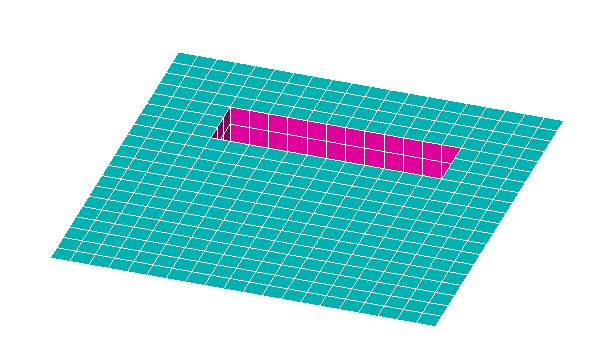
\includegraphics[scale=0.5]{trincheira.png}
\end{figure}
\end{frame}

%------------------------------------------------

\begin{frame}
\frametitle{O Problema}
\begin{itemize}
\item Implementação fornecida era sequencial
\item Para 4000 elementos de malha, o tempo total era de 167s
\item Objetivo: Encontrar as rotinas mais custosas e otimizá-las
\item Subrotina mais custosa: \texttt{Ghmatecd}
\begin{itemize}
 Constrói as matrizes $H$ \& $G$ do problema dinâmico
\end{itemize}
\end{itemize}
\end{frame}

%------------------------------------------------

\begin{frame}
\frametitle{O Problema}
Construir as seguintes matrizes:

\[
 H, G = 
\left[ 
\begin{array}{c@{}c@{}c@{}c}
  \textcolor{red}{
  \left(\begin{array}{ccc}
         . & . & .\\
         . & . & .\\
         . & . & .\\
  \end{array}\right)} & 

  \left[\begin{array}{ccc}
         . & . & .\\
         . & . & .\\
         . & . & .\\
  \end{array}\right] &

  \left[\begin{array}{ccc}
         . & . & .\\
         . & . & .\\
         . & . & .\\
  \end{array}\right] & 

  \left[\begin{array}{ccc}
         . & . & .\\
         . & . & .\\
         . & . & .\\
  \end{array}\right] & \\

  \left[\begin{array}{ccc}
         . & . & .\\
         . & . & .\\
         . & . & .\\
  \end{array}\right] & 
  
  \textcolor{red}{
  \left(\begin{array}{ccc}
         . & . & .\\
         . & . & .\\
         . & . & .\\
  \end{array}\right)} & 

  \left[\begin{array}{ccc}
         . & . & .\\
         . & . & .\\
         . & . & .\\
  \end{array}\right] &

  \left[\begin{array}{ccc}
         . & . & .\\
         . & . & .\\
         . & . & .\\
  \end{array}\right] & \\

  \left[\begin{array}{ccc}
         . & . & .\\
         . & . & .\\
         . & . & .\\
  \end{array}\right] & 

  \left[\begin{array}{ccc}
         . & . & .\\
         . & . & .\\
         . & . & .\\
  \end{array}\right] &

  \textcolor{red}{
  \left(\begin{array}{ccc}
         . & . & .\\
         . & . & .\\
         . & . & .\\
  \end{array}\right)} & 

  \left[\begin{array}{ccc}
         . & . & .\\
         . & . & .\\
         . & . & .\\
  \end{array}\right] & \\
\end{array}\right]
\]

\end{frame}

%-----------------------------------------------

\begin{frame}
\begin{algorithm}[H]
\label{ghmatecd_old}
\caption{Creates $H, G \in \Cfield^{(3m)\times(3n)}$}
\begin{algorithmic}[1]
	\Procedure{Ghmatecd}{}
		\For{$j := 1, n$} 
			\For{$i := 1, m$}
				\State{$ii := 3(i-1) + 1$ }   
				\State{$jj := 3(j-1) + 1$ }
				\If{$i == j$}
					\State{\textcolor{red}{$Gelement, Helement \leftarrow \text{Sing\_de}(i)$}}					
				\Else
					\State{$Gelement, Helement \leftarrow \text{Nonsingd}(i, j)$}	
				\EndIf
				\State{$G[ii:ii+2][jj:jj+2] \leftarrow Gelement$}
				\State{$H[ii:ii+2][jj:jj+2] \leftarrow Helement$}
			\EndFor
	 \EndFor
	\EndProcedure
\end{algorithmic}
\end{algorithm}
Como paralelizar com OpenMP?
\end{frame}

%------------------------------------------------

\begin{frame}
\begin{algorithm}[H]
\label{ghmatecd_openmp}
\caption{Creates $H, G \in \Cfield^{(3m)\times(3n)}$}
\begin{algorithmic}[1]
	\Procedure{Ghmatecd}{}
		\State{\textcolor{blue}{\text{\#pragma omp parallel for collapse(2)}}}
		\For{$j := 1, n$} 
			\For{$i := 1, m$}
				\State{$ii := 3(i-1) + 1$ }   
				\State{$jj := 3(j-1) + 1$ }
				\If{$i == j$}
					\State{\textcolor{red}{$Gelement, Helement \leftarrow \text{Sing\_de}(i)$}}					
				\Else
					\State{$Gelement, Helement \leftarrow \text{Nonsingd}(i, j)$}	
				\EndIf
				\State{$G[ii:ii+2][jj:jj+2] \leftarrow Gelement$}
				\State{$H[ii:ii+2][jj:jj+2] \leftarrow Helement$}
			\EndFor
	 \EndFor
	\EndProcedure
\end{algorithmic}
\end{algorithm}
E na GPU?
\end{frame}

%------------------------------------------------

\begin{frame}
\frametitle{O Problema}
\begin{itemize}
\item \texttt{Nonsingd} e \texttt{Sing\_de} computam uma integral numericamente

\begin{equation}
	\int_{a}^{b} f(x)\text{d}x \approx \sum_{i = 1}^{g}w_i f(x_i) \label{quadrature} \nonumber
\end{equation}

\item Em nosso caso, avaliar $f(x)$ em um ponto $x_i$ é custoso.
\item Uma forma de paralelizar esta rotina é fazer uma redução

\end{itemize}
\end{frame}

%------------------------------------------------

%\begin{frame}
%\frametitle{O Problema}
Expandindo a rotina \textcolor{orange}{\texttt{Nonsingd}}, temos:

%\begin{algorithm}[H]
%\algsetup{linenosize=\tiny}
\scriptsize
\label{ghmatecd_new}
\begin{algorithmic}[1]
	\Procedure{Ghmatecd\_nonsingd}{}
		\For{$j := 1, n$} 
			\For{$i := 1, m$}
				\State{$ii := 3(i-1) + 1;     jj := 3(j-1) + 1$}
				\State{Allocate \textit{Hbuffer} \& \textit{Gbuffer}, buffer of matrices $3 \times 3$ of size $g^2$}
				\textcolor{orange}{
				\If{$i \neq j$}
					\For{$y := 1, g$}
						\For{$x := 1, g$}
							\State{$\textit{Hbuffer}(x, y) \leftarrow \text{GenerateMatrixH}(i, j, x, y)$}
							\State{$\textit{Gbuffer}(x, y) \leftarrow \text{GenerateMatrixG}(i, j, x, y)$}
						\EndFor
					\EndFor
				\EndIf
				\State{$Gelement \leftarrow \text{SumAllMatricesInBuffer}(\textit{Gbuffer})$} 
				\State{$Helement \leftarrow \text{SumAllMatricesInBuffer}(\textit{Hbuffer})$}
				}
				\State{$G[ii:ii+2][jj:jj+2] \leftarrow Gelement$}
				\State{$H[ii:ii+2][jj:jj+2] \leftarrow Helement$}
			\EndFor
	 \EndFor
	\EndProcedure
	\Procedure{Ghmatecd\_Sing\_de}{}
	\textcolor{red}{	
	\For{$i := 1, m$}
			\State{$ii := 3(i-1) + 1$}
			\State{$Gelement, Helement \leftarrow \text{Sing\_de}(i)$}	
			\State{$G[ii:ii+2][ii:ii+2] \leftarrow Gelement$}
			\State{$H[ii:ii+2][ii:ii+2] \leftarrow Helement$}
	 \EndFor
     }
	\EndProcedure
	\Procedure{Ghmatecd}{} 
		\State{$\text{Ghmatecd\_Nonsingd}()$}
		\State{$\text{Ghmatecd\_Sing\_de}()$}
	\EndProcedure
		
\end{algorithmic}
%\end{algorithm}

%\end{frame}

%------------------------------------------------

%------------------------------------------------
\normalsize

\begin{frame}
\frametitle{Estratégia}
\begin{itemize}
\item Aloque uma \textit{thread} para cada ponto da quadratura
	\begin{itemize}
	\item Como a integral é sobre um elemento quadrilateral, temos $g \times g$ pontos
	\item A soma gerará uma matriz $3 \times 3$
\[
  \underbrace{
  \left[\begin{array}{ccc}
         . & . & .\\
         . & . & .\\
         . & . & .\\
  \end{array}\right]
  }_{\text{Final}}
    =
  \underbrace{ 
  \left[\begin{array}{ccc}
         . & . & .\\
         . & . & .\\
         . & . & .\\
  \end{array}\right]
  }_{\text{Thread 1}}
    +
  \underbrace{
  \left[\begin{array}{ccc}
         . & . & .\\
         . & . & .\\
         . & . & .\\
  \end{array}\right]
  }_{\text{Thread 2}}
    +
   \cdots
    +
  \underbrace{
  \left[\begin{array}{ccc}
         . & . & .\\
         . & . & .\\
         . & . & .\\
  \end{array}\right]
  }_{\text{Thread } g \times g}

\]

\item Armazene as fatias na memória compartilhada
\item Some

\end{itemize}

\end{itemize}
\end{frame}

%------------------------------------------------

\begin{frame}
\frametitle{O Problema}

\[
 H, G = 
\left[ 
\begin{array}{c@{}c@{}c@{}c}
  \textcolor{red}{
  \left(\begin{array}{ccc}
         . & . & .\\
         . & . & .\\
         . & . & .\\
  \end{array}\right)} & 

  \left[\begin{array}{ccc}
         . & . & .\\
         . & . & .\\
         . & . & .\\
  \end{array}\right] &

  \left[\begin{array}{ccc}
         . & . & .\\
         . & . & .\\
         . & . & .\\
  \end{array}\right] & 

  \left[\begin{array}{ccc}
         . & . & .\\
         . & . & .\\
         . & . & .\\
  \end{array}\right] & \\

  \left[\begin{array}{ccc}
         . & . & .\\
         . & . & .\\
         . & . & .\\
  \end{array}\right] & 
  
  \textcolor{red}{
  \left(\begin{array}{ccc}
         . & . & .\\
         . & . & .\\
         . & . & .\\
  \end{array}\right)} & 

  \left[\begin{array}{ccc}
         . & . & .\\
         . & . & .\\
         . & . & .\\
  \end{array}\right] &

  \left[\begin{array}{ccc}
         . & . & .\\
         . & . & .\\
         . & . & .\\
  \end{array}\right] & \\

  \left[\begin{array}{ccc}
         . & . & .\\
         . & . & .\\
         . & . & .\\
  \end{array}\right] & 

  \left[\begin{array}{ccc}
         . & . & .\\
         . & . & .\\
         . & . & .\\
  \end{array}\right] &

  \textcolor{red}{
  \left(\begin{array}{ccc}
         . & . & .\\
         . & . & .\\
         . & . & .\\
  \end{array}\right)} & 

  \left[\begin{array}{ccc}
         . & . & .\\
         . & . & .\\
         . & . & .\\
  \end{array}\right] & \\
\end{array}\right]
\]

\end{frame}

%----------------------------------------------

\begin{frame}
\begin{itemize}
\item Aloque um bloco para cada matrix $3 \times 3$

\[
\left[ 
\begin{array}{c@{}c@{}c@{}c}
  \textcolor{red}{
    B_{1,1}
  } & 
    B_{1,2}
    &
    B_{1,3}
    &
    B_{1,4} & \\
    
    B_{2,1} &
  
  \textcolor{red}{
    B_{2,2}
  } &
    B_{2,3}
    &
    B_{2,4} & \\
     
    B_{3,1}
   & 
    B_{3,2}
    &
   \textcolor{red}{
    B_{3,3}
   }
    &
    B_{3,4}
    & \\
\end{array}\right]
\]

\item Compute os elementos da diagonal principal (\textcolor{red}{em vermelho}) na CPU
\begin{itemize}
	A diagonal tem menos elementos
\end{itemize}

\end{itemize}
\end{frame}
%-----------------------------------------------

\begin{frame}
\frametitle{Testes}
\begin{itemize}
	\item Todos os testes executados em precisão simples
	\item Foram utilizados 8 pontos de gauss, totalizando 64 \textit{threads} por bloco
	\item Verificamos que $||H_{cpu} - H_{gpu}||_1 < 10^{-4}$ e $||G_{cpu} - G_{gpu}||_1 < 10^{-4}$
	\item Todos os experimentos foram executados $30$ vezes
	\item Processador: AMD A10-7700K; GPU: GeForce GTX980

\end{itemize}

\end{frame}

%------------------------------------------------
\begin{frame}

\begin{figure}[ht]
\centering
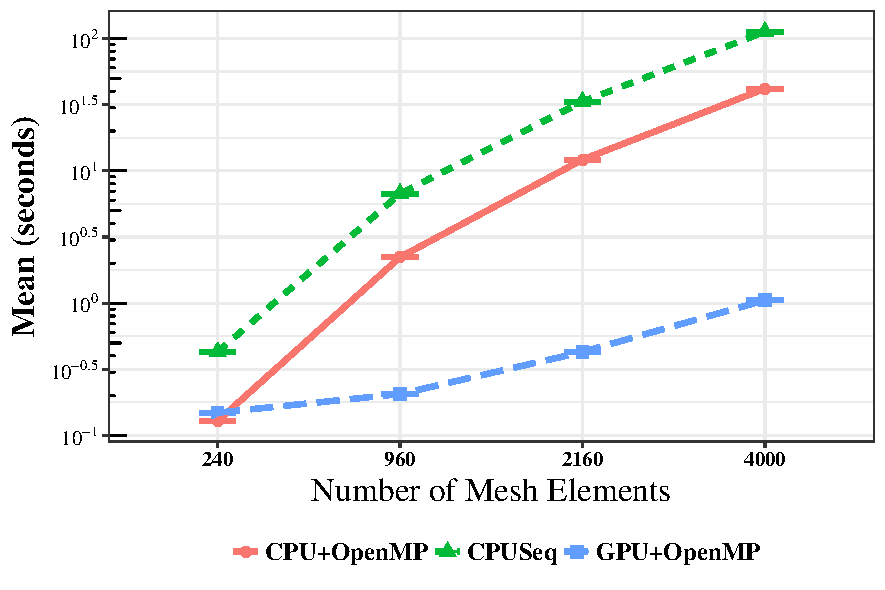
\includegraphics[scale=0.7]{results1.pdf}
\label{fig:graphic1}
\end{figure}

\end{frame}
%------------------------------------------------

\begin{frame}
\frametitle{Fim}
\center{\Large{Obrigado!}}
\scriptsize

Agradecemos a CAPES pela minha bolsa de IC a a Nvidia pela doação da GPU que usamos
\normalsize
\end{frame}


\end{document} 
